\subsection{有限生成投射模的局部刻画}

定理 1. 设 A 是一个环，P 是一个 A-模。下列性质等价：

\begin{enumerate}
\def\labelenumi{(\alph{enumi})}
\item
  \(\mathbf{P}\) 是一个有限生成投射模。
\item
  \(\mathbf{P}\) 是一个有限表示模，且对每个极大理想 \(\mathfrak{m}\)（\(\mathbf{A}\) 的），\(\mathbf{P}_{\mathfrak{m}}\) 是一个自由 \(\mathbf{A}_{\mathfrak{m}}\) -模。
\item
  P 是一个有限生成模，对一切 \(p \in \text{Spec}(A)\)，\(A_{p}\) -模 \(P_{p}\) 是自由的，且若记其秩为 \(r_{p}\)，则函数 \(p \mapsto r_{p}\) 在拓扑空间 \(\text{Spec}(A)\) 中是局部常值的（也就是说，\(\text{Spec}(A)\) 的每个点都有一个使该函数为常值的邻域）。
\item
  存在元素的有限族 \((f_{i})_{i\in \mathbf{I}}\)（\(\mathbf{A}\) 的），生成理想 \(\mathbf{A}\)，使对一切 \(i\in \mathbf{I}\)，\(\mathbf{A}_{f_i}\) -模 \(\mathbf{P}_{f_i}\) 是有限秩自由的。
\item
  对 A 的每个极大理想 m，存在 \(f \in A - m\) 使 \(P_{f}\) 是有限秩自由 \(A_{f}\) -模。
\end{enumerate}

我们通过证明下述蕴含格式来证明该定理

\pandocbounded{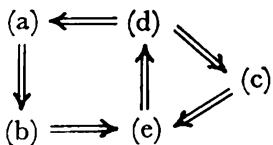
\includegraphics[keepaspectratio]{images/part001_f1dfd2f3.jpg}}

\begin{enumerate}
\def\labelenumi{(\alph{enumi})}
\item
  \(\Rightarrow\) (b): 我们知道有限生成投射模是有限表示的（第 I 章 §2 第 8 节引理 8 (iii)）；若 P 是投射 A-模，则 \(P_{m} = P \otimes_{A} A_{m}\) 是投射 \(A_{m}\) -模（《代数》第 II 章 §5 第 1 节命题 4 的推论）；最后，由于 \(A_{m}\) 是局部环，每个有限表示的投射 \(A_{m}\) -模都是自由的（§3 第 2 节命题 5 的推论）。
\item
  \(\Rightarrow\) (e): 这由第 1 节命题 2 的推论得出。
\item
  \(\Rightarrow\) (e): 设 \(m\) 是 \(A\) 的一个极大理想；记 \(r_m = n\)，并设 \((x_i)_{1 \leqslant i \leqslant n}\) 是 \(P_m\) 的一个基。我们可以假设诸 \(x_i\) 是元素 \(p_i \in P\)（\(1 \leqslant i \leqslant n\)）的典范像（至多相差 \(A_m\) 的一个可逆元的乘法）。设 \((e_i)_{1 \leqslant i \leqslant n}\) 是 \(A^n\) 的典范基，\(u: A^n \to P\) 是使 \(u(e_i) = p_i\)（对 \(1 \leqslant i \leqslant n\)）成立的同态。由于 \(P\) 是有限生成的，由第 1 节命题 2，存在 \(f \in A - m\) 使 \(u_f\) 是满射。我们得出 \(u_{fg}\) 对一切 \(g \in A - m\) 也是满射，且按假设存在 \(g \in A - m\) 使 \(r_p = n\) 对 \(p \in X_g\) 成立。于是把 \(f\) 换成 \(fg\)，我们可以假设 \(r_p = n\) 对一切 \(p \in X_f\) 成立。于是 \(u_p: A_p^n \to P_p\) 是满射同态，且 \(P_p\) 与 \(A_p\) 是同秩的自由 \(A_p\) -模；因而（§3 第 2 节命题 6 的推论）\(u_p\) 对一切 \(p \in X_f\) 是双射。设 \(p'\) 是 \(A_f\) 的一个素理想，\(p\) 是它在典范映射下在 \(A\) 中的逆像；若把 \((A_f^n)_{p'}\) 与 \((P_f)_{p'}\) 在典范同构下分别等同于 \(A_p^n\) 与 \(P_p\)，则 \((u_f)_{p'}\) 等同于 \(u_p\)，从而是双射。我们得出 \(u_f\) 是双射（§3 第 3 节定理 1），这就确立了 (e)。
\item
  \(\Rightarrow\) (d): 设 E 是 \(f\in A\)（使 \(\mathbf{P}_f\) 为有限生成自由 \(\mathbf{A}_f\) -模者）组成之集。假设蕴含 E 不含于 A 的任何极大理想，因而 E 生成理想 A，从而存在 E 中元素的有限族 \((f_{i})_{1 \leqslant i \leqslant n}\) 与 \(a_{i} \in \mathbf{A}\)（\(1 \leqslant i \leqslant n\)）使 \(1 = \sum_{i=1}^{n} a_{i} f_{i}\)；由此得 (d)。
\item
  \(\Rightarrow\) (c): 由第 1 节命题 3 的推论，P 是有限生成的。另一方面，对 A 的每个素理想 p，存在指标 \(i\) 使 \(\mathfrak{p} \in \mathrm{X}_{f_i}\)；若 \(\mathfrak{p}' = \mathfrak{p}_{f_i}\)，则 \(\mathrm{P}_{\mathfrak{p}} = (\mathrm{P}_{f_i})_{\mathfrak{p}'}\)（§2 第 5 节命题
\end{enumerate}

\begin{enumerate}
\def\labelenumi{\arabic{enumi})}
\setcounter{enumi}{9}
\tightlist
\item
因而按假设 \(\mathbf{P}_{\mathfrak{p}}\) 是自由的且与 \(\mathbf{P}_{f_i}\) 同秩，这就证明了 (c)。
\end{enumerate}

\begin{enumerate}
\def\labelenumi{(\alph{enumi})}
\setcounter{enumi}{3}
\tightlist
\item
  \(\Rightarrow\) (a): 考虑环 \(\mathbf{B} = \prod_{i\in I}\mathbf{A}_{f_i}\) 与 B-模
\end{enumerate}

\[
\mathbf {M} = \prod_ {i \in I} \mathrm{P} _ {f _ {i}} = \mathrm{P} \otimes_ {\mathbf {A}} \mathrm{B}.
\]

对每个指标 \(i\)，存在自由 \(\mathbf{A}_{f_i}\) -模 \(\mathbf{L}_i\) 使 \(\mathbf{P}_{f_i}\) 是 \(\mathbf{L}_i\) 的一个直因子，并且可以假设所有 \(\mathbf{L}_i\) 有相同的秩；则

\(L = \prod_{i \in I} L_i\) 是一个自由 B-模，M 是它的一个直因子，换言之 M 是一个有限生成投射 B-模。由于 B 是忠实平坦 A-模（第 1 节命题 3），我们得出 P 是一个有限生成投射 A-模（第 I 章 §3 第 6 节命题 12）。

推论 1. 设定理 1 陈述中的等价性质成立。设 \(m\) 是整数 \(>0\)，使得对 \((x_{i})_{1\leqslant i\leqslant m}\)（\(\mathbf{P}\) 的元素的族）的每一个，存在 \((a_{i})_{1\leqslant i\leqslant m}\)（\(\mathbf{A}\) 的元素的族），它们不全是零因子且使 \(\sum_{i=1}^{m} a_i x_i = 0\)。则对一切 \(p \in \operatorname{Spec}(A)\)，\(r_p \leqslant m\)。

设 \(p\) 是 \(A\) 的一个素理想；记 \(r = r_p\)，并设 \((y_j)_{1 \leqslant j \leqslant r}\) 是自由 \(\mathbf{A}_{p}\) -模 \(\mathbf{P}_{p}\) 的一个基。存在元素 \(x_j\)（\(1 \leqslant j \leqslant r\)，属于 \(\mathbf{P}\)）与 \(s \in A - p\) 使 \(y_j = x_j / s\) 对一切 \(j\) 成立。于是对每个元素族 \((a_j)_{1 \leqslant j \leqslant r}\)（\(A\) 的），若满足 \(\sum_{j=1}^{r} a_j x_j = 0\)，则 \(\sum_{j=1}^{r} (a_j / 1) y_j = 0\)（在 \(P_p\) 中），从而 \(a_j / 1 = 0\) 对 \(1 \leqslant j \leqslant r\) 成立。由于 \(A - p\) 不包含 0，这表明诸 \(a_j\) 都是 \(A\) 中的零因子（\(\S 2\) 第 1 节注 3），因而必然 \(r \leqslant m\)。

推论 2. 每个有限表示的平坦模都是投射模.\par

若 P 是一个有限表示的平坦 A-模而 m 是 A 的一个极大理想，则 \(A_{m}\) -模 \(P_{m}\) 是平坦的（§3 第 4 节命题 13）且有限表示的（§2 第 4 节），从而是自由的（§3 第 2 节命题 5 的推论 2），于是定理 1 的条件 (b) 成立。

注

\begin{enumerate}
\def\labelenumi{(\arabic{enumi})}
\item
  存在非投射的有限生成平坦模（习题 7）。
\item
  定理 1 的推论 2 可推广到非交换环上的模（第 I 章 §2 习题 15）。
\end{enumerate}
% semantic-fragments: legacy-input-seam
\relax{}
